\section{Experiment and Result Analysis}
In this section, MQTT and Modbus are chosen as our target protocols from a variety of ICPs in the experiment. The test cases, which are generated by HexGANFuzzer and the control group, are used to stress test the target and trigger anomalies of the ICP.% We generate large amounts of test cases by our generative model. Then the generated data is used to stress test the target and trigger anomalies of the ICP. Finally,  according to the anomalies triggered, vulnerabilities in the anomalies will be submitted for the improvement of the ICP after analysis. We evaluate various aspects of performance of our method by experimentation. 
% to find the reason for the target anomalies

%\subsection{Environment construction of MQTT and Modbus}
%To show the effectiveness and efficiency of our framework, we apply it to test MQTT, one of the mainstream ICPs. To indicate the versatility of our method, another ICP, Modbus, is also used to test.
%
%\subsubsection{MQTT}
%MQTT (Message Queuing Telemetry Transport) protocol is an application layer ICP based on publication and subscription under the ISO (International Organization for Standardization) standard and works on the TCP/IP protocol cluster. It is simple to implement, provides the transmission data with the quality of service, has the characteristics of lightweight, high bandwidth utilization efficiency, data independence and so on. The message format of MQTT is illustrated in Fig. \ref{FigMQTTFormat}.  
%
%\begin{figure}[htbp]   %  插入一栏图片
%	\centering 
%	\includegraphics[width=\textwidth]{Figure/FigMQTTFormat.eps}
%	\caption{Message format of MQTT}
%	\label{FigMQTTFormat}
%\end{figure}
%
%In the experiment, we utilize Mosquitto v1.5.8 \cite{light2017mosquitto} as the open-source message broker of message push ICP MQTT v3.1 and  Paho-MQTT v1.0.2 \cite{light2017mosquitto} as the MQTT client. 
%
%\subsubsection{Modbust-TCP}
%There are many variants of Modbus, including Modbus-TCP, Modbus-UDP and so on. We choose Modbus-TCP as another fuzzing ICP in this study. It uses master-slave communication mode, in which the master communicates with slaves by actively sending data frames \cite{swales1999open}. 
% and receiving 

\subsection{Evaluation Setup}
%\subsubsection{Experimental Environment}
% one of the popular deep learning framework in the industrial community,

%To improve the training efficiency, we
Tensorflow is adopted to implement the model architecture. We train our model  and launch the fuzzing attack on the same machine with 8 processors (Intel(R) Core (TM) i7-6700K CPU@4.00GHz)  16.0GB memory (RAM) Nvidia GeForce GTX 1080 Ti (11GB) and 64-bit ubuntu16.04, x64-based processor. In the experiment, we utilize Mosquitto v1.5.8 \cite{light2017mosquitto} as the open-source message broker of message push ICP MQTT v3.1 and  Paho-MQTT v1.0.2 as the MQTT client.

%we initialize all weights from zero-centered Normal distribution with a standard deviation of 0.2, which can increase diversity to a certain extent. T
As for the parameter setting, the mini-batch size is set to 64 in all models based on a large amount of training data. The $keep\_prob$ hyperparameter of dropout is set to 0.7. The learning rate of Generator and Critic is set to 0.0001 and 0.0004 in the Adam optimizer. $\lambda$ in the loss equation of Critic is 10. The dimension of the initial noise $zd$ is 50 and feature dimension $dm$ is 80. The repeat times of the transfomer block is 4 and the number of heads is 2. We train the models for 100 epochs and save the generator model for every 10 epochs to get plentiful test cases.

% When launching an attack, the simulators run on another machine with 4 processors (Intel (R) Core (TM) i5-5300U CPU@2.30GHz) 16.00GB memory (RAM) and 64-bit Microsoft Windows 10 Professional Operating System, x64-based processor.

%\subsubsection{Model Training Setting}
%As for the parameter setting, we initialize all weights from zero-centered Normal distribution with a standard deviation of 0.2, which can increase diversity to a certain extent. The mini-batch size is set to 32 in all models based on a large amount of training data. The $keep\_prob$ hyperparameter of dropout is set to 0.7. The learning rate of G and D is set to 0.0001 and 0.0004 in the Adam optimizer. As to the checkpoint in the generative model, the interval of model saving frequency is set to 10. We train the models for 100 epochs and save the generator model for every 10 epochs to get plentiful test cases.
%\subsubsection{Model Training Setting}

%\begin{figure}[htbp]   %  插入一栏图片
%	\centering 
%	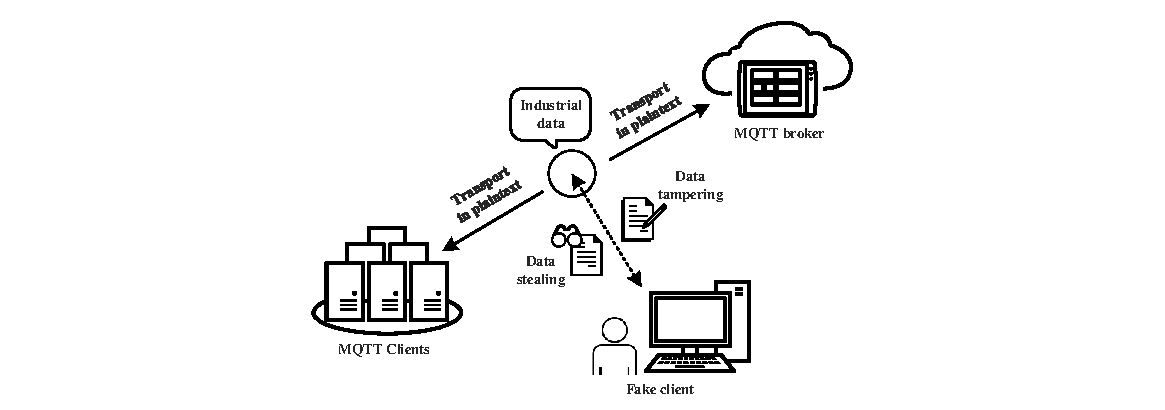
\includegraphics[width=\textwidth]{Figure/FigMQTTEnvironment.eps}
%	\caption{MQTT enviroment}
%	\label{FigMQTTEnvironment}
%\end{figure}

\begin{figure*}[t] 		 %  插入双栏图片
	\centering
	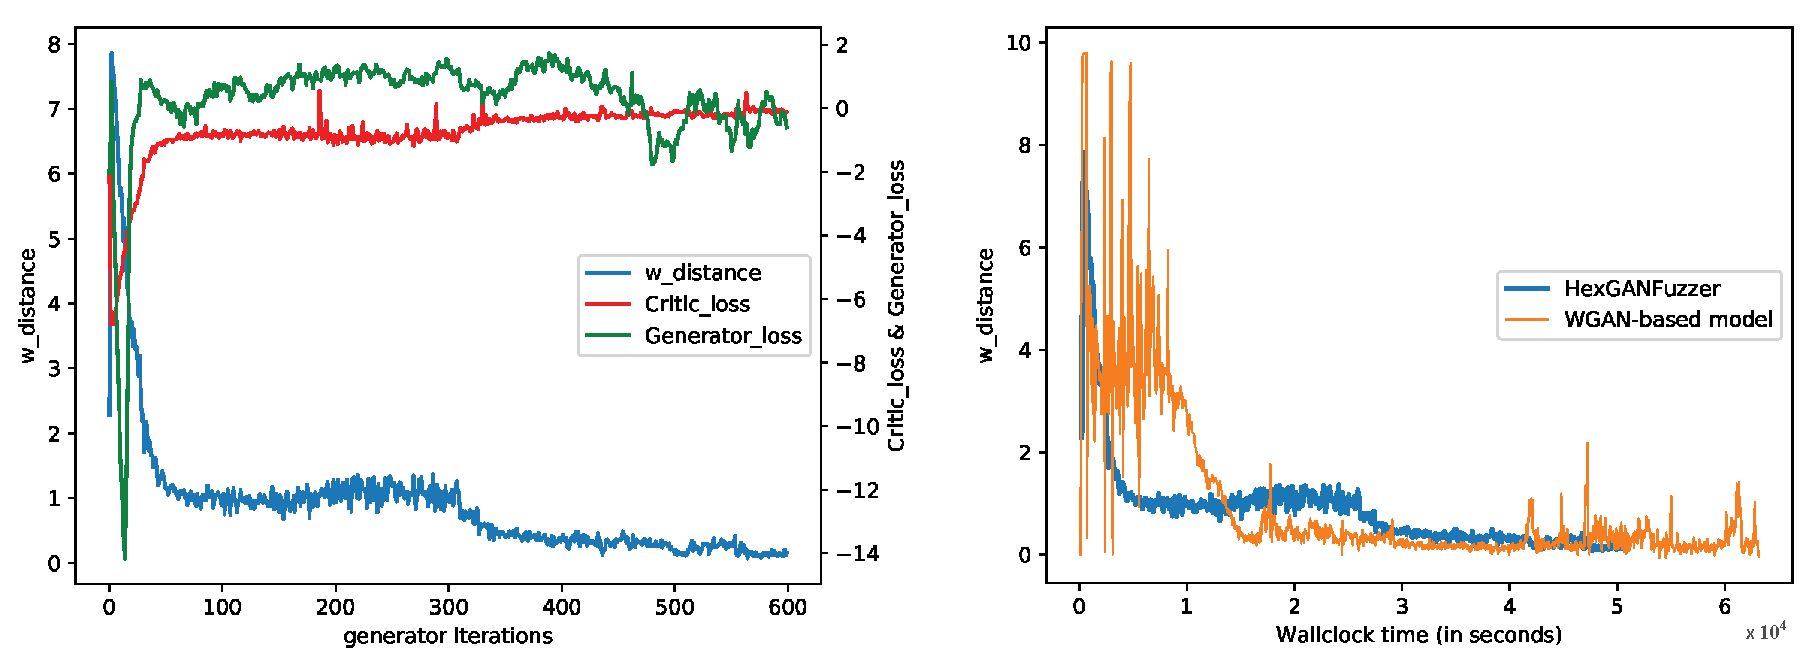
\includegraphics[width=\textwidth]{Figure/FigModelW-distance.eps}
	\caption{Dataset(500,000 test cases) W-distance over generator iterations (left) or wall-clock time (right) for HexGANFuzzer}
	\label{FigModelW-distance}
\end{figure*} 

\subsection{Fuzz Testing The Target ICP}
One advantage of our method over GANs is largely overcoming the problem of unstable training of GANs, such as non-convergence, vanishing gradient and mode collapse. % We design our model architecture based on these architectural constraints and improve training speed and sample quality. 
%  with Wasserstein distance and gradient penalty 
To demonstrate this, we train HexGANFuzzer on a dataset with 500,000 test cases and plot Wasserstein distance and losses of the generator and the critic in Fig. \ref{FigModelW-distance} (left). For comparision, we train another WGAN-based model with the same hyperparameter setting. The result in Fig. \ref{FigModelW-distance} (right) represents that our method converges faster and is more stable at convergence.

With the trained model, we generate test cases. Then the generate test cases are input to the system under test, and we implement the fuzzy test process according to the standard fuzzy test process.

%In the process of inputting test cases into ICSs under test, we monitor the system in real time. If anomalies occur in the process, such as the output clobber problems and interface crash, we record and restart the test process at the current point. At the end of the entire test, we analyze the causes of antecedent anomalies and the logs of server systems to find the running status of potential vulnerabilities. 


%In order to capture the MQTT communication data, an MQTT network environment based ICS is prepared as illustrated in Fig. \ref{FigMQTTEnvironment}.

%\subsubsection{Model Training}

%\subsubsection{Training Data}
%Training data in deep learning significantly influence model training. In the experiment, training data about the two industrial control protocols is collected separately. 
%
%\begin{figure}[htbp]   %  插入一栏图片
%	\centering 
%	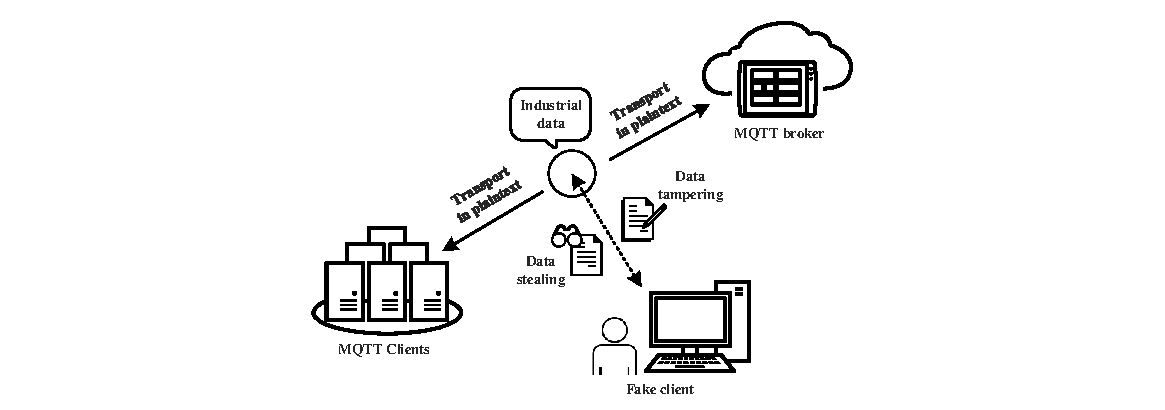
\includegraphics[width=\textwidth]{Figure/FigMQTTEnvironment.eps}
%	\caption{MQTT enviroment}
%	\label{FigMQTTEnvironment}
%\end{figure}
%
%\quad \textit{\textbf{a. MQTT.}}
%In order to capture the MQTT communication data, an MQTT network environment based ICS is prepared as illustrated in Fig. \ref{FigMQTTEnvironment}. Wireshark \cite{orebaugh2006wireshark} is applied to grab packets during communication. These grabbed frames serve as the training data for the HexGANFuzzer framework. 
%After fetching the connection information between the legal clients and the MQTT broker, we construct a disguised MQTT client to send the same connection information to connect to the broker in the IoT network with no authentication security measures. The disguised MQTT client launches the attack by sending fake MQTT messages which are generated by fuzzy test models. 
%
%\quad \textit{\textbf{b. Modbus-TCP.}}
%Pymodbus \cite{collins2013pymodbus}, a python package that implements the Modbus protocol, is used to generate the training data frames. Enough different types of data frames can be generated quickly via Pymodbus, which is practical and convenient. In the experiment, a Modbus-TCP implementation, Modbus RSSim v8.20, is applied as the fuzzing targets. The generated test cases are sent to the Modbus-TCP implementation by a python script over sockets to test the effects in simulated applications.



%weight clipping

%Following the setting in the subsection Model Training Setting, we train one model with the same optimizer (Adam) and learning rate as WGAN with weight clipping. The results also represent that our method converges faster and is more stable at convergence.

%\subsubsection{Logging and Evaluation}
%Logging is the basis for further analysis of model performance and fuzzing effectiveness. By analyzing logs of the communication process is an effective method to find ICPs’ anomalies. Some vulnerabilities may be manifested according to the obvious abnormal behavior of the system, and some behaviors need to be further analyzed. Based on the statistical analysis of the log file, we evaluate experimental results. Furthermore, we artificially analyze specific anomalies to get more details. Test data that causes target anomalies will be recollected and put into the training data set again. Data augmentation and value mutation operation will be applied to these data before putting it into the retraining data set. The retrained model with these mutated data can improve the capability of the model to detect vulnerabilities.

\subsection{Result Analysis}
In this part, we show the experimental results in three aspects. We first reveal statistical results and their analysis. Then we present a special anomaly that occurred in the process of fuzzing MQTT implementations. Lastly, to show the methodology’s protocol independence in fuzz testing of ICPs, the result of testing Modbus-TCP is presented.

\subsubsection{Results and Statistical Analysis}
The widely used General Purpose Fuzzer (GPF) \cite{demott2007revolutionizing}, CNN-1D model, LSTM-based seq2seq model, and WGAN-based model are chosen as fuzzers in the control group in this study. After fuzzers in the experimental group and control group are fully trained, fuzz testing is conducted by sending a total of 100,000 generated test cases to MQTT implementations through the TCP/1883 port. According to the three aforementioned evaluation metrics, the details of different models are as follows. 

%According to the three aforementioned evaluation metrics, the effectiveness and efficiency of our fuzzing framework HexGANFuzzer and fuzzers in the control group are evaluated and represented graphically. Details are as follows.  

%\begin{table*}[t]
%	\centering
%	\caption{Performance Metrics Comparison}
%	\label{F-measure}
%	\renewcommand{\arraystretch}{0.8}
%	\begin{tabular}{ m{50pt}<{\centering} |m{70pt}<{\centering}|m{30pt}<{\centering}|m{60pt}<{\centering}|m{40pt}<{\centering}|m{40pt}<{\centering}|m{40pt}<{\centering}}
%		\toprule
%		\textbf{Dataset
%			(number of training cases)} & \textbf{Methods}          & \textbf{Year} & \textbf{F-measure} & \textbf{SE}     & \textbf{SP}     & \textbf{AC}     \\ \midrule
%		& GPF              & 2007 & --         & 0.5252 & 0.5798 & 0.6474 \\ \cmidrule(l){2-7} 
%		& CNN-1D model     & 2014 & 0.6701    & 0.8437 & 0.9743 & \textbf{0.8626} \\ \cmidrule(l){2-7} 
%		10,000  & LSTM-based model & 2018 & 0.6300    & \textbf{0.8563}   & 0.9007 & 0.8254 \\ \cmidrule(l){2-7} 
%		& WGAN-based model & 2019 & 0.7960    & 0.7696 & 0.9115 & 0.8165 \\ \cmidrule(l){2-7} 
%		& HexGANFuzzer      & 2020 & \textbf{0.8208}    & 0.8274 & \textbf{0.9775} & 0.8608 \\ \midrule
%		& GPF              & 2007 & --         & 0.5720 & 0.5730 & 0.6510 \\ \cmidrule(l){2-7} 
%		& CNN-1D model     & 2014 & 0.8373    & \textbf{0.8670} & 0.9842 & 0.8690 \\ \cmidrule(l){2-7} 
%		500,000 & LSTM-based model & 2018 & 0.8388    & 0.8203 & \textbf{0.9856} & 0.8700 \\ \cmidrule(l){2-7} 
%		& WGAN-based model & 2019 & 0.8396    & 0.8108 & 0.9371 & 0.8906 \\ \cmidrule(l){2-7} 
%		& HexGANFuzzer      & 2020 & \textbf{0.8502}    & 0.8538 & 0.9478 & \textbf{0.9271} \\ \bottomrule
%	\end{tabular}
%\end{table*}

\begin{table*}[t]
	\centering
	\caption{Performance comparison with different dataset size (The number of training cases are 10k/500k).} 
	% higher SE shows a higher rate of function codes being generated correctly; higher SP shows a higher rate of non-essential hexadecimal characters being generated correctly; higher AC shows a higher rate of the overall message packages being generated correctly.
	\label{F-measure}
	\renewcommand{\arraystretch}{1.5}
	\begin{threeparttable}
	\begin{tabular}{c|c|c|c|c}
		\hline
		\textbf{Models}          & \textbf{SE$^{\rm a}$} & \textbf{SP$^{\rm a}$}     & \textbf{AC$^{\rm b}$}     & \textbf{F-measure$^{\rm c}$}     \\ \hline
		GPF               &  52.52\%/57.20\% & 57.98\%/57.30\% & 64.74\%/65.10\%  & --/-- \\ [3pt]
		\hline
		CNN-1D     &  84.37\%/\textbf{86.70\%}    & 97.43\%/98.42\% & \textbf{86.26\%}/86.90\% &  67.01\%/83.73\% \\ [3pt]
		\hline
		LSTM  &    \textbf{85.63\%}/82.03\%  &  90.07\%/\textbf{98.56\%}  &82.54\%/87.00\%  &  63.00\%/83.88\%\\ [3pt]
		\hline
		WGAN &    76.96\%/81.08\%   & 91.15\%/93.71\%& 81.65\%/89.06\% & 79.60\%/83.96\% \\ [3pt]
		\hline
		HexGANFuzzer      &  82.74\%/85.38\%    &  \textbf{97.75\%}/94.78\%& 86.08\%/\textbf{92.71\%} & \textbf{82.08\%}/\textbf{85.02\%} \\ [3pt]
		\hline
	\end{tabular}
	\begin{tablenotes}
		\item[a] SE/SP corresponds to the rate of function codes/non-essential hexadecimal characters being generated correctly.
		\item[b] AC is the comprehensive embodiment of SE and SP.
		\item[c] F-measure indicates a harmonic mean that function codes and the overall message packages are generated correctly, which is the embodiment of model learning ICPs' specification ability.
	\end{tablenotes}
\end{threeparttable}
\end{table*}

% , and the Sensitivity of this method is 5.78\% higher than the WGAN-based model.

\textit{\textbf{a. F-measure.}} Table \ref{F-measure} shows the accuracy of each method in generating legitimate test cases on a dataset of 10,000 and 500,000 training data. It can be observed from the table that the algorithm in this paper has higher scores of Sensitivity, Accuracy and F-measure than other models in the control group in datasets of different sizes. Although the Sensitivity of the CNN-1D model and LSTM-based seq2seq model is higher than our model, the types of test cases generated are relatively single. And the algorithm in this paper has the highest F-measure. For the dataset of 10,000 training data, the F-measure of generating legitimate test cases reaches 82.08\%, which is 2.48\% higher than the second highest model. On the dataset of 500,000 training data, our method is 1.06\% higher in F-measure and 3.65\% higher in Accuracy than the second highest model. 

Therefore, we can draw a conclusion from the evaluation metrics of the performance of machine learning models in table \ref{F-measure}: in terms of datasets with different data sizes, the model in this paper is superior to other fuzzy test case methods in each evaluation metric of generating legitimate test cases.


\textit{\textbf{b. EVD.}}
%In order to map the EVD value of each model to a relatively small scope for diagrammatic comparison, we normalize all EVD values under the same iteration through Z-score standardization. 
The experimental results of EVD are shown in Fig. \ref{FIGURE_EVD}. Due to not involving a continuously learning process, the performance of GPF has a downward trend on the targets when compared to the other four fuzzing models based on depth learning. From the perspective of the aforementioned five models, the performance of the EVD indicators is: GPF $\textless$ CNN-1D model $\approx$ LSTM-based model $\textless$ WGAN-based model $\textless$ HexGANFuzzer. 

% \begin{figure}[t]
% 	\centering
% 	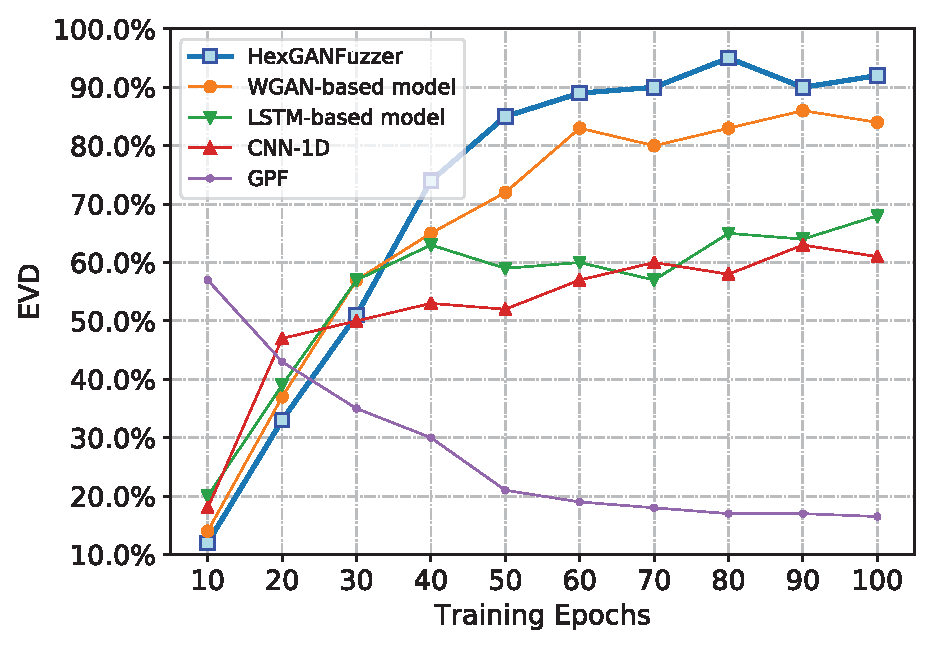
\includegraphics[width=\textwidth]{Figure/FIGURE_EVD.eps}
% 	\caption{EVD changes with the training epochs}
% 	\label{FIGURE_EVD}
% \end{figure}



%generative adversarial
After training more than 30 epochs, the EVD rates of deep learning algorithms obviously exceed the GPF algorithm. With the rising trends of rates slow down significantly after 50 epochs, the average EVD rates of CNN-1D model and LSTM-based model are 60\% to 70\% compared with 75\% to 90\% of generative adversarial algorithms, which may be caused by the inability to learn a hierarchy of representations of the data effectively. For the generative adversarial algorithms from 50 to 100 epochs, the average EVD rate of HexGANFuzzer is approximately 8\% higher than the WGAN-based model, which indirectly indicates that HexGANFuzzer is more applicable to test cases generation for ICPs. %Due to the unsupervised characteristic of generative adversarial algorithms, it may result in generating a large number of malformed protocol message sequences, leading to normal throwing which may cause EVD can not be further promoted.  %as presented in Table \ref{Triggered_Anomalies_HexGANFuzzer}
It's worth going into detail that our trained model can effectively detect kinds of anomalies, which shows we are likely to achieve the higher code coverage and the stronger ability of our model has to detect anomalies.
%Usually, the richer the data type, the higher code coverage we are likely to achieve, and the stronger ability a model has to detect anomalies.
%\begin{table}[htbp]
%	\caption{Triggered Anomalies and Triggered Frequency of HexGANFuzzer}
%	\label{Triggered_Anomalies_HexGANFuzzer}
%	\centering
%	%
%	\begin{tabular}{m{100pt}<{\centering}  m{40pt}<{\centering} m{50pt}<{\centering} }
%		\toprule
%		\bfseries Triggered Anomalies &  \bfseries Frequency (Times) & \bfseries ATITA (Mins)\\
%		\midrule
%		Using abnormal function code & 104 & 5.78\\
%		Data length unmatched & 121 & 4.52\\
%		Integer overflow & 21 & 13.46 \\
%		Broker memory overflow & 2 & 285.05 \\
%		Unknown attack & 53 &10.64\\
%		\bottomrule
%	\end{tabular}
%\end{table}

%where Frequency represents the number at which the specified type of anomalies is triggered by the model during test time and average time interval of triggered anomalies (ATITA) is the quotient of the number of triggered anomalies and test time.
\begin{figure}[t]
	\centering
	\begin{minipage}[t]{0.48\textwidth}
		\centering
		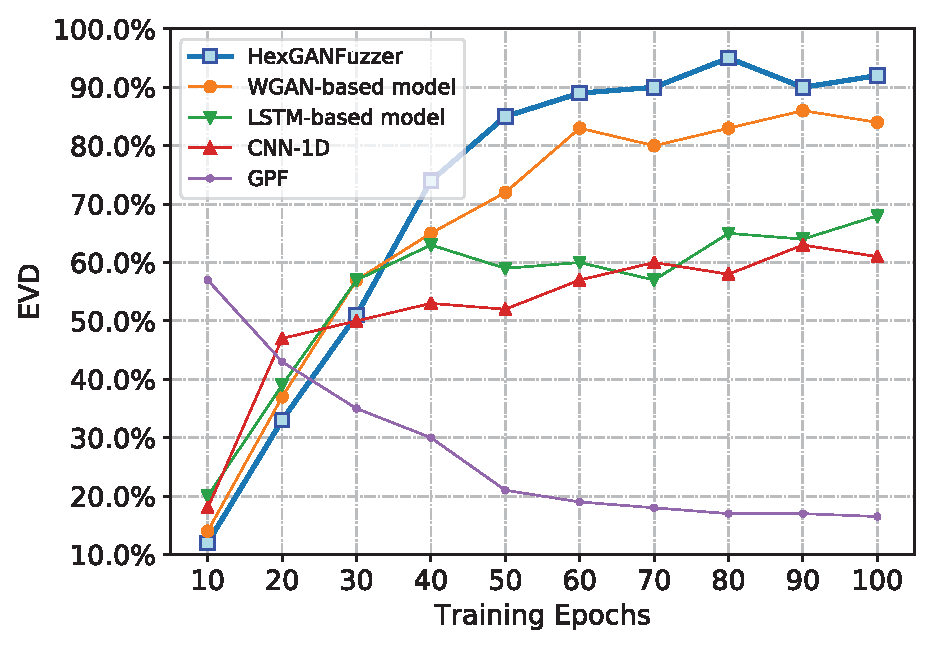
\includegraphics[width=6cm]{Figure/FIGURE_EVD.eps}
		\caption{EVD changes with the training epochs}
		\label{FIGURE_EVD}
	\end{minipage}
	\begin{minipage}[t]{0.48\textwidth}
		\centering
		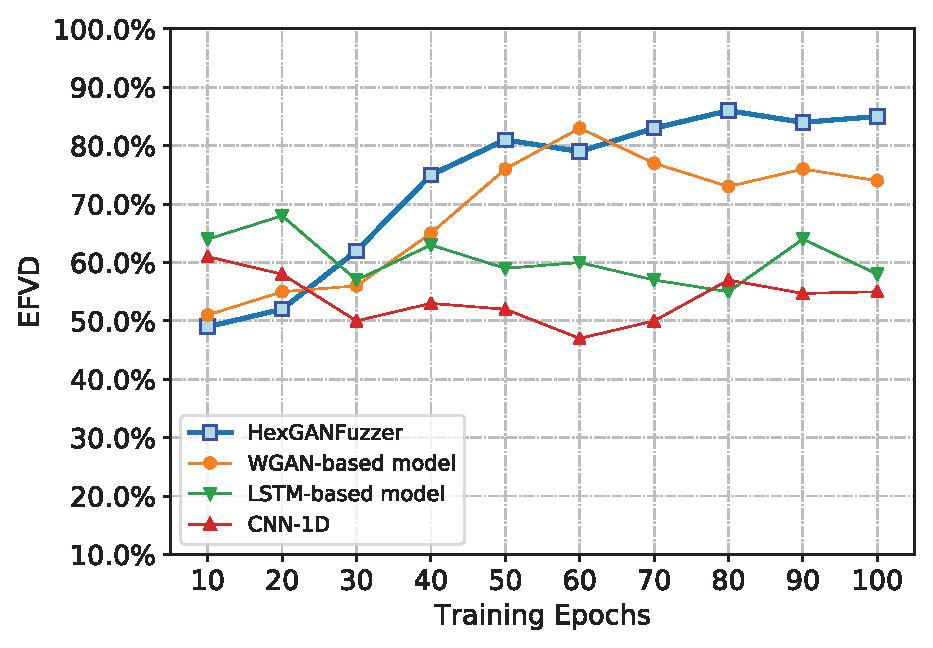
\includegraphics[width=6cm]{Figure/FIGURE_EFVD.eps}
		\caption{EFVD changes with the training epochs}
		\label{FIGURE_EFVD}
	\end{minipage}
\end{figure}
\textit{\textbf{c. EFVD.}}
%There is a huge difference in the training time of different GPF and the time of anomalies triggered by GPF is constant under different iterations, so it is not discussed in this part. The normalization is applied to EFVD, which is the same as the EVD. The testing depth has increased as illustrated in Fig. \ref{FIGURE_EVD}. % at the expense of reducing the code coverage of fuzz testing
%But what makes a difference, rather, is that high test efficiency is maintained on the premise of attaining high EVD rates. The variation trend of EFVD of different deep learning based models is presented in Fig. \ref{FIGURE_EFVD}. 
There is a huge difference in the training time of different GPF, so it is not discussed in this part. It can be seen from Fig. \ref{FIGURE_EFVD} that when doing less training epochs, models with relatively short training time can achieve higher EFVD scores. And with the deepening of training, TAT values of different models become more and more different, so models with higher potential efficiency of vulnerability detection will get higher EFVD scores. Looking at the overall trend, the average EFVD score of our model is 19.45\% higher than that in the CNN-1D model, 15.14\% higher than the LSTM-based model and 5.26\% higher than the WGAN-based model. And the fluctuation of our model is relatively small, which indicates that our model can maintain relatively stable efficiency on the basis of balancing TT and TAT.

\subsubsection{Potential Vulnerabilities Found}
Due to the limited space, we mainly talk about one exception that we analyzed, which is \textit{\textbf{Buffer Exception}}. 
% When the mosquitto broker receives message frames from the client, it will store data into the buffer. And it will parse the message frames based on the MQTT protocol grammar without checking the whole message length. 
The broker truncates the message frames according to the reamining length in the MQTT protocol only. The part of the data that exceeds the remaining length will be left in the buffer, which will cause the problem of no answering of the following message frames.


\begin{figure*}  %  插入一栏图片
	\centering 
	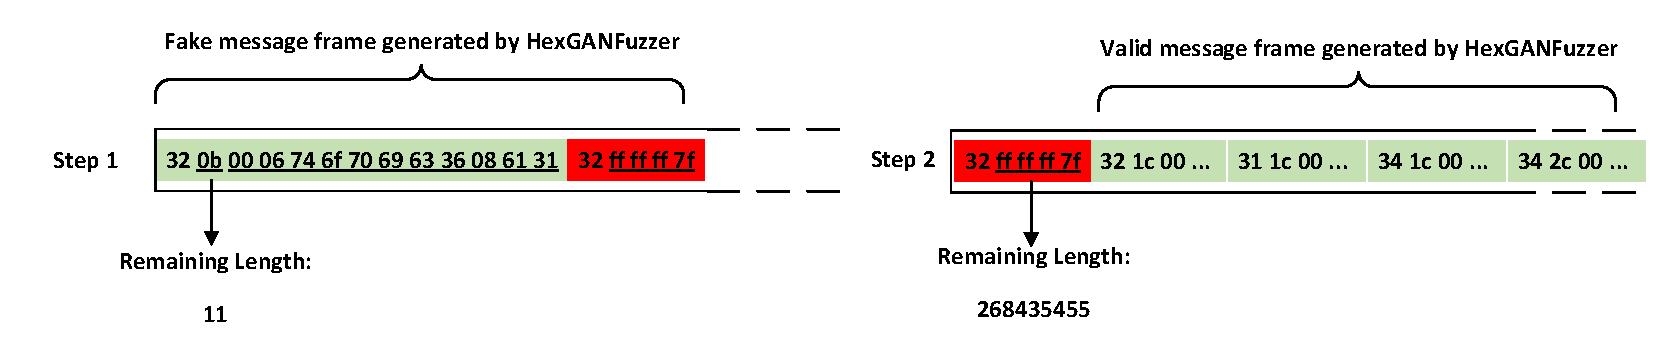
\includegraphics[width=\textwidth]{Figure/FigHexGANFuzzer_BufferException.eps}
	\caption{Potential vulnerabilities analysis}
	\label{FigHexGANFuzzer_BufferException}
\end{figure*}
As the Fig. \ref{FigHexGANFuzzer_BufferException} shows, in $step1$, we send the generated message frames formed by green and red box part to the broker.
% where the green box part is a complete MQTT message frame and the red box part is additional.
% The mixed message frame is stored in the buffer first. Then, the broker only parses the green part of the message frames correctly and 
The red part is left in the buffer of the MQTT broker. In this situation, the broker has treated \textbf{0x32ffffff7f} as the part of the message header of the next message frame. In $step2$, when the next real message frames arrived at the buffer, the broker has considered 268 million as the remaining length of this message frame. 
% It means the following message frames in green boxes and the previous red part should form a message frame with a length of about 268 million. 
This makes the communication invalid between the client and the broker for a period of time unless the buffer is full or the length of the message frames reach 268 million.


\subsubsection{Applying The Method to Modbus-TCP}


As shown in Table \ref{table_MQTT}, we detect these potential vulnerabilities in Modbus-TCP via the new trained HexGANFuzzer. 
%including slave crash, station off-line, using abnormal function code and so on,
\begin{table}[htbp]
	\caption{Potential Vulnerabilities and  in Modbus-TCP}
	\label{table_MQTT}
	\centering
	% \begin{tabular} {p{100pt}<{\centering} p{40pt}<{\centering} p{50pt}<{\centering}}
	\begin{tabular}{ccc}
		\toprule
		\makecell[tl]{\bfseries Triggered Anomalies} &  {\bfseries NTA} & {\bfseries ATITA (Mins)} \\
		\midrule
		\makecell[tl]{Slave crash}  & {29 times} & 21.11 \\
		\makecell[tl]{Station ID xx off-line} & {164 times} & 0.79 \\
		\makecell[tl]{Using abnormal function code}  & {207 times} & 0.52 \\
		\makecell[tl]{Automatically closes window}  & {13 times} & 28.47 \\
		\makecell[tl]{Data length unmatched}  & {190 times} & 0.63\\
		\makecell[tl]{Unknown attack}  & {197 times} & 0.59 \\
		\bottomrule
	\end{tabular}
\end{table}

The number of Triggered anomalies (NTA) represents the total number of anomalies triggered by the models during test time and average time interval of triggered anomalies (ATITA) is the quotient of the number of triggered anomalies and test time. Experiments on the Modbus-TCP protocol prove that our method has great versatility. % In the experiment, we send the generated data messages $S_i$ to the slave stations and record the corresponding received message $R_i$. Massive message pairs $<S_i, R_i>$ are obtained. According to the abnormal protocol characterization above, we analyze and compare the specified field values and obtained the following statistical results. % {350pt}{lcc}



%where Frequency represents the number at which the specified type of anomalies is triggered by the model during test time and average time interval of triggered anomalies (ATITA) is the quotient of the number of triggered anomalies and test time.


